\documentclass[a4paper]{article}
\usepackage[utf8]{inputenc}
\usepackage[spanish]{babel} 
\renewcommand{\spanishtablename}{Tabla} 
\spanishdecimal{.}
\usepackage{verbatim}
\usepackage{amssymb}
\usepackage{subcaption}
\usepackage{wrapfig}
\usepackage{graphicx}
\usepackage{hyperref}
\usepackage{mathtools}
\usepackage{float}
\usepackage{siunitx}
\usepackage[utf8]{inputenc}
\renewcommand{\thefootnote}{\arabic{fotnote}}
\setlength{\parskip}{\baselineskip} 
\usepackage{pdfpages}

\begin{document}

\begin{titlepage}
\paragraph{}

\begin{center}
\vspace*{0.10in}
\begin{figure}
\raggedleft

\includegraphics[scale=0.12]{unam.png}
\hspace{7.2cm}
\raggedright

\includegraphics[scale=0.15]{fac.png}    
\end{figure}
\vspace*{0.5in}
UNIVERSIDAD NACIONAL AUTÓNOMA DE MÉXICO\\
\vspace*{0.2in}
FACULTAD DE CIENCIAS \\
\vspace*{0.5in}
\begin{large}
Laboratorio de Calor, Ondas y Fluidos\\
\end{large}
\vspace*{0.2in}
\begin{Large}
\textbf{Práctica 6} \\
\textbf{Relación Presión-Profundidad} \\
\end{Large}
\vspace*{0.3in}
\vspace*{0.3in}
\rule{80mm}{0.1mm}\\
\vspace*{0.1in}
\begin{large}
Profesor:  Quintanar Robles, Luis  \\
Ayudante: Quintanar Cortés, Luis Enrique \\
Mesa 1\\
Fecha de la práctica: 24 de Septiembre de 2019.\\
Alumnos: León Arenal Sebastian.\\
Robledo Ibarra Emiliano. \\
Toledo Castañeda Akim Tarik.\\

\end{large}
\end{center}
\end{titlepage}



\section*{Resumen.}
Se buscó una relación entre la presión y la profundidad a la que se sumerge un cuerpo y para ello se midió la diferencia de altura entre las columnas de un manómetro de alcohol y como éstas cambian al introducir un tubo de vidrio, conectado por una manguera al manómetro, en tres distintos fluidos. Con estos datos se encontró una relación lineal entre el cambio de alturas  y la profundidad (diferencia entre profundidades y altura de una columna)  obteniendo las siguientes pendientes: $m_{aceite}=1.07\pm0.03$, $m_{shampoo}=1.19\pm0.03$ y $m_{glicerina}=1.518\pm0.017$. Se observa que estas pendientes son muy similares al cociente de densidades (densidades relativas) que se comprobaron por medio de valores medidos directamente con un densimetro.


\section*{Introducción.}
Los fluidos siempre han sido tema de estudio, pues cada fluido posee ciertas características que lo definen y diferencian de otros. Aspectos como su densidad, calor específico y viscosidad definen algunas de las características únicas de cada fluido. La presión es una medida que nos indica como una fuerza es aplicada sobre un cuerpo y se define como la magnitud de la fuerza aplicada por unidad de área $[1]$; definimos dos tipos de presión: absoluta y manométrica. La presión absoluta se debe a la presión que ejerce la atmósfera sobre la superficie terrestre y afecta a todos los cuerpos dentro de la atmósfera. La presión manométrica es aquella que se encuentra dentro de un sistema aislado, sin efecto de la presión atmosférica $[2]$. 

El objetivo de la práctica consistió en encontrar una relación entre la presión al interior de un líquido y su alteración debida a las alturas (en este caso profundidades) utilizadas. Se verificó la reproducibilidad del experimento; esto se realizó aprovechando la presión atmosférica y manométrica, de forma que se pudiera  comparar y medir la presión hidrostática (que es la fuerza por unidad de área que un fluido, ejerce sobre un cuerpo sumergido dentro del mismo $[1]$). Para poder determinar la relación se midieron diferencias de alturas ocasionadas por la presión, tanto en un medidor de un manómetro como en una punta prueba. Según la teoría la relación de presiones está dada por:

\begin{equation}
    P_{atm} + \rho_{fluido}gh = P_{atm} + \rho_{alcohol}g\Delta h + \rho_{fluido}gL
\end{equation}

Denotando a $P_{atm}$ como la presión atmosférica, $\rho_{fluido}gh$ como la presión que ejerce el fluido a una profundidad h, $\rho_{alcohol}g\Delta h$ la presión que se obtiene del manómetro diferencial, $\rho_{fluido}gL$ la presión que ejerce una columna del fluido con altura L. Se buscará una comparación entre la descripción de dicha ecuación con los datos obtenidos y se verificará si es realmente una buena descripción del fenómeno estudiado, además se comprobara si de dicha relación se puede extraer información como la densidad del fluido.

En cuanto a las hipótesis utilizadas, se dio por hecho que el líquido que se utilizo se encontraba en reposo lo cual permitió poder medir sin alteraciones del movimiento del fluido, de manera similar se omitió la ley de Snell, debido a que al estar en medios distintos la luz cambia su ángulo de refracción (vidrio, aire y líquido) pero al estar al borde cerca de las paredes de la probeta el ángulo se volvía despreciable y por tanto resultaba lo mismo medir directamente la columna por fuera en lugar de meter la cinta métrica y dañarla o llenarla de algún líquido. En general se buscó reducir el contenido extra de líquido dentro de la punta prueba por lo que se utilizó la hipótesis sobre como este líquido, que alteraba la medida, dejaba de influir en la presión después de cierto lapso de tiempo (de uno a dos minutos y dependiendo del líquido) ya que después de este el líquido extra fluía hacia abajo. Como las hipótesis se utilizaron para simplificar las mediciones, estas influyen directamente en la medida, sin embargo, no son lo suficientemente grandes como para omitir o sesgar la medición ya que al trabajar con aparatos con reducida resolución como el manómetro o un flexómetro los mismos instrumentos truncan la posible obtención de las medidas, de esta manera conociendo que las hipótesis sobre las mediciones no afectan en gran medida los datos recabados, así el único requerimiento que se cuidó que se cumpliese fue el reposo del líquido por lo cual el reporte se limita a líquidos en reposo. Se utlilizó la hipótesis que dentro del manómetro había alcohol etílico puro con $789 kg/m^3$[3] como densidad del alcohol dentro del manómetro.

\section*{Procedimiento.}
Para las relaciones que se buscaron encontrar, se midieron de las alturas que realizaron tres fluidos distintos: glicerina, aceite y shampoo. A manera de no contaminar cada recipiente con un liquido distinto, se intercambió todo el sistema probeta-manguera con otros equipos del laboratorio y además, como medida de precaución adicional, el responsable de manejar dichos instrumentos se lavó las manos antes y después de manipular cada fluido para así no contaminar los demás y manejarlos debidamente. También se procuró que el fluido no permeara más allá de la manguera, evitando así que el manómetro se contaminara. De esta forma se construyó una extensión de un manómetro utilizando un capilar de vidrio conectado a una manguera que funcionaría de punta prueba [Figura 1].

\begin{figure}[H]
\centering
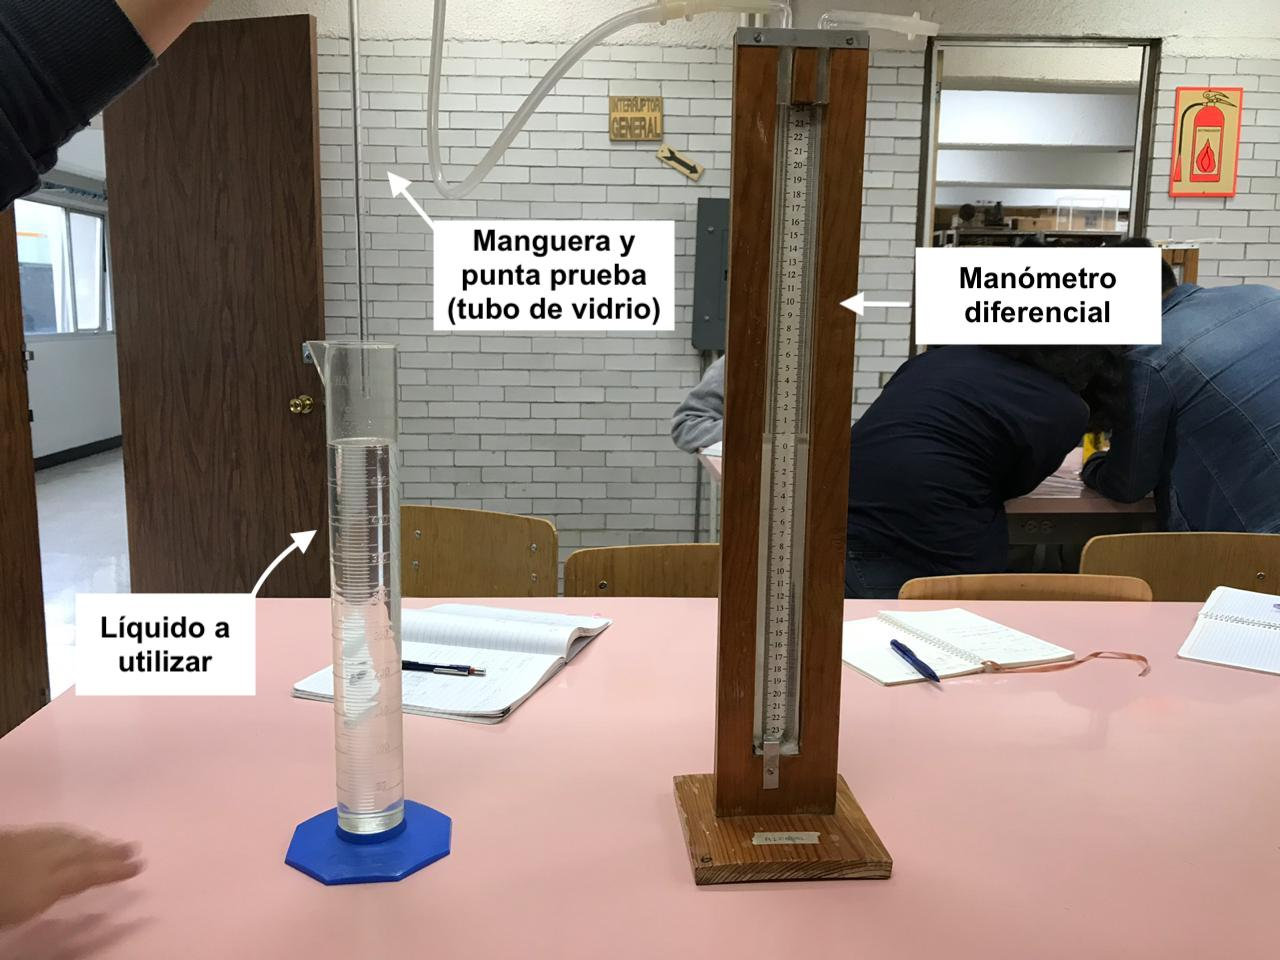
\includegraphics[scale=0.2]{manometro.jpeg}
\caption{Dispositivo utilizado para las mediciones, un manómetro y su extensión para medir.}
\end{figure}

Una vez unidas las partes del sistema se comenzó a medir cada marca de 50 mL de la probeta, es necesario aclarar que estas medidas sólo funcionaron de referencia para poder determinar un punto sin tener que marcar el material, de forma que se sumergió hasta la marca deseada y posterior a ello se realizaron las medidas de: $\Delta l$ la diferencia de alturas del manómetro, $h$ la profundidad de la punta prueba y $l$ la altura de la columna que penetró la punta prueba. Se comenzaron las mediciones desde la parte más alta y se siguió un esquema como el siguiente: se realizaron las  mediciones bajando dos marcas y posterior a ello se repitió la primera de estas para poder observar su reproducibilidad. En resumen, se bajaban dos y se subía a la primera de ellas y se iteraba el proceso. Se dictaminó de dicha forma ya que así sería menor la cantidad de fluido que subiría por la columna y de esta forma afectar lo menos posible a la medición ya que al penetrar dentro del capilar (punta prueba) la permanencia del mismo material podría variar la medición puesto que este fluido que baja a través de las paredes también ejerce una presión hidrostática. En cuanto al manómetro, se buscó tomar mediciones basadas en el menisco, debido a que en algunas ocasiones era necesario discernir si era óptimo redondear hacia el entero más bajo o el más alto, se optó por redondear (en caso de que fuera necesario) el menisco de la izquierda al entero menor y el de la derecha al mayor de forma que se evitaran ambigüedades y los errores se distribuyeran.

Se midieron diez veces cada altura y se repitieron para cada una de forma que se realizaron 60 mediciones en total, de las cuales sólo se verán reflejadas la mitad debido a que la otra parte se utilizó de comprobación en cuanto a reproducibilidad refiere. En cuanto al tratamiento de datos se tomaron la profundidad a la cual se sumergió la punta ($h$) y se le restó la longitud de la columna interna ($L$) para después poder graficar esta medida contra la diferencia en alturas del manómetro.


Para poder otorgar una incertidumbre adecuada a cada medición se notó que en el manómetro al obtener la altura de la columna se midieron dos cantidades directas y se operó con ellas de forma que su incertidumbre se sumó, y por tanto $\Delta l$ cuenta con incertidumbre $0.1 cm$; tanto la profundidad de la punta prueba y la altura de la columna se midieron directamente al pegarlo a la pared interna por lo cual ambos contaron con incertidumbre de $0.05 cm$. Por último para la diferencia entre profundidad y altura de la columna, ya que solamente se restaron dos elementos con la misma incertidumbre se le asoció el doble de la misma, esto es $h-l$ es decir, una  incertidumbre de $0.1 cm$.

\section*{Resultados.}
En esta sección se colocan los datos que se denotan:
\begin{itemize}
    \item $h$: la profundidad a la cual se sumergió la punta prueba.
    \item $L$: la longitud de la columna interna.
    \item $\Delta l$: diferencia en alturas del manómetro.
\end{itemize}

\subsection*{Aceite}

% Table generated by Excel2LaTeX from sheet 'Aceite'
\begin{table}[H]
  \centering
    \begin{tabular}{|c|c|c|} \hline
    Profundidad \textbf{h} [cm] & Longitud de columna interna \textbf{L} [cm] & Diferencia alturas manómetro \textbf{$\Delta l$} [cm]\\ \hline
    2.70$\pm0.05$  & 1.50$\pm0.05$  & 1.5$\pm0.1$ \\ \hline
    5.80$\pm0.05$  & 3.00$\pm0.05$  & 3.1$\pm0.1$ \\ \hline
    8.80$\pm0.05$  & 4.40$\pm0.05$  & 4.8$\pm0.1$ \\ \hline
    11.60$\pm0.05$ & 5.80$\pm0.05$  & 6.7$\pm0.1$ \\ \hline
    14.70$\pm0.05$ & 7.00$\pm0.05$  & 8.4$\pm0.1$ \\ \hline
    17.10$\pm0.05$ & 8.40$\pm0.05$  & 10.4$\pm0.1$ \\ \hline
    20.50$\pm0.05$ & 9.70$\pm0.05$  & 12.2$\pm0.1$ \\ \hline
    23.50$\pm0.05$ & 11.00$\pm0.05$ & 14.0$\pm0.1$ \\ \hline
    26.40$\pm0.05$ & 12.40$\pm0.05$ & 15.9$\pm0.1$ \\ \hline
    30.00$\pm0.05$ & 13.30$\pm0.05$ & 17.3$\pm0.1$ \\ \hline
    \end{tabular}%
    \caption{Datos obtenidos con la probeta llena de aceite}
\end{table}%

\begin{figure}[H]
    \centering
    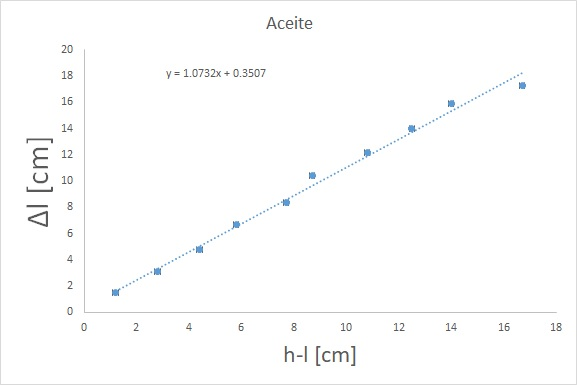
\includegraphics[width=12cm]{GRF-A.jpg}
    \caption{Comparación h-L contra diferencia de alturas en el manómetro}
\end{figure}

Del cual se obtuvo: $m_{aceite}=1.07\pm0.03$, que se multiplicó con el valor de la densidad del alcohol para obtener la densidad del líquido, por lo que el valor es: $850 \pm 20 kg/m^3$. Que en comparación del medido directamente $900. \pm 5 kg/m^3$


\subsection*{Shampoo}

% Table generated by Excel2LaTeX from sheet 'Shampoo'
\begin{table}[H]
  \centering
    \begin{tabular}{|c|c|c|} \hline
    Profundidad \textbf{h} [cm] & Longitud de columna interna \textbf{L} [cm] & Diferencia alturas manómetro \textbf{$\Delta l$} [cm] \\ \hline
    3.10$\pm0.05$  & 1.40$\pm0.05$  & 2.0$\pm0.1$ \\ \hline
    6.00$\pm0.05$  & 2.40$\pm0.05$  & 4.7$\pm0.1$ \\ \hline
    8.00$\pm0.05$  & 3.50$\pm0.05$  & 6.3$\pm0.1$ \\ \hline
    11.10$\pm0.05$ & 4.70$\pm0.05$  & 8.7$\pm0.1$ \\ \hline
    14.70$\pm0.05$ & 6.40$\pm0.05$  & 10.6$\pm0.1$ \\ \hline
    17.50$\pm0.05$ & 7.60$\pm0.05$  & 12.6$\pm0.1$ \\ \hline
    20.70$\pm0.05$ & 9.00$\pm0.05$  & 14.5$\pm0.1$ \\ \hline
    23.60$\pm0.05$ & 10.30$\pm0.05$ & 16.5$\pm0.1$ \\ \hline
    26.60$\pm0.05$ & 11.80$\pm0.05$ & 18.6$\pm0.1$ \\ \hline
    29.40$\pm0.05$ & 12.80$\pm0.05$ & 19.7$\pm0.1$ \\ \hline
    \end{tabular}%
    \caption{Datos obtenidos con la probeta llena de shampoo}
\end{table}%


\begin{figure}[H]
    \centering
    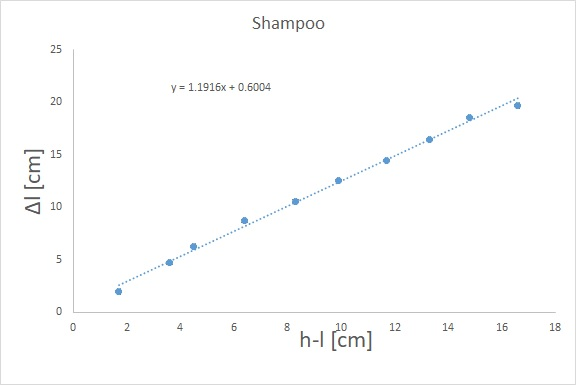
\includegraphics[width=12cm]{GRF-Sh.jpg}
    \caption{Comparación h-L contra diferencia de alturas en el manómetro}
\end{figure}

Del cual se obtuvo: $m_{shampoo}=1.19\pm0.03$ que cuando se multiplica por la densidad del alcohol so obtiene $940\pm20 kg/m^3$ contra el valor directo de $1030.\pm5 kg/m^3$


\subsection*{Glicerina}

% Table generated by Excel2LaTeX from sheet 'Glicerina'
\begin{table}[H]
  \centering
    \begin{tabular}{|c|c|c|} \hline
    Profundidad \textbf{h} [cm] & Longitud de columna interna \textbf{L} [cm] & Diferencia alturas manómetro \textbf{$\Delta l$} [cm] \\ \hline
    2.40$\pm0.05$  & 1.20$\pm0.05$  & 1.8$\pm0.1$ \\ \hline
    5.20$\pm0.05$  & 3.00$\pm0.05$  & 3.7$\pm0.1$ \\ \hline
    8.00$\pm0.05$  & 4.30$\pm0.05$  & 5.8$\pm0.1$ \\ \hline
    10.80$\pm0.05$ & 5.80$\pm0.05$  & 7.8$\pm0.1$ \\ \hline
    13.60$\pm0.05$ & 7.30$\pm0.05$  & 10.0$\pm0.1$ \\ \hline
    16.60$\pm0.05$ & 8.50$\pm0.05$  & 12.2$\pm0.1$ \\ \hline
    19.30$\pm0.05$ & 10.20$\pm0.05$ & 14.3$\pm0.1$ \\ \hline
    22.30$\pm0.05$ & 11.70$\pm0.05$ & 16.4$\pm0.1$ \\ \hline
    25.30$\pm0.05$ & 13.10$\pm0.05$ & 18.5$\pm0.1$ \\ \hline
    27.60$\pm0.05$ & 14.30$\pm0.05$ & 20.4$\pm0.1$ \\ \hline
    \end{tabular}%
    \caption{Datos obtenidos para la probeta llena de glicerina}
\end{table}%

\begin{figure}[H]
    \centering
    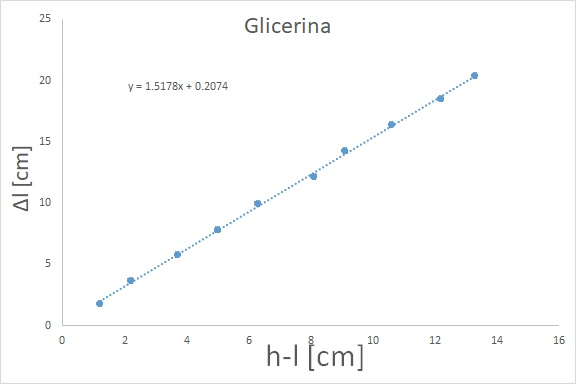
\includegraphics[width=12cm]{GRAF-Gli.jpg}
    \caption{Comparación h-L contra diferencia de alturas en el manómetro}
\end{figure}

Del cual se obtuvo: $m_{glicerina}=1.517\pm0.017$. Y al multiplicarlo por la densidad del alcohol, se obtiene la densidad experimental (indirecta) de la glicerina: $1197\pm13 kg/m^3$. Contra el valor directo: $1260.\pm5 kg/m^3$.

\newpage
\section*{Conclusiones.}

Las relaciones obtenidas son congruentes con la teoría, al graficar los datos, se hace presente una forma lineal y esta concuerda con los datos obtenidos, de esta manera se confirma que es una muy buena descripción utilizar el modelo de presión hidrostática que la teoría predice. En cuanto a las pendientes obtenidas, para la glicerina se obtuvo $m_{glicerina}=1.518\pm0.017$, para el shampoo $m_{shampoo}=1.19\pm0.03$ y para el aceite de oliva $m_{aceite}=1.07\pm0.03$. 

Si pensamos a estos cocientes como la densidad relativa, al hacer los cocientes de densidades (Fluido/Alcohol) se obtuvieron: $940\pm20 kg/m^3$ para el shampoo, $1197\pm13 kg/m^3$ para la glicerina y $850 \pm 20 kg/m^3$ para el aceite. Según la teoría, la ecuación:
\begin{equation}
    (h-L)\frac{\rho_{fluido}}{\rho_{alcohol}}=\Delta l
\end{equation}

dicta que que las rectas encontradas experimentalmente deberían tener una pendiente igual al cociente de densidades (Fluido/Alcohol). En efecto, comparando el cociente con las pendientes obtenidas experimentalmente se observa que son muy similares. Debido a la precisión con la que se registraron los datos es probable que la diferencia entre los datos teóricos y experimentales se deban a un error en la densidad supuesta del alcohol, se concluyó que el alcohol dentro del manómetro puede estar contaminado (en este caso con una densidad mayor) ya que no se proporcionó más información de la sustancia contenida dentro del instrumento mas que una etiqueta en la base del manómetro que decía "alcohol".

En cuanto a las hipótesis podemos ver que no solamente facilitaron las mediciones sino que su repercusión es mínima y podemos sustentar esto gracias a que las medidas y cálculos hechos con estas son congruentes bajo el modelo que se quiso comprobar; las densidades obtenidas después de operar son congruentes y la diferencia entre las medidas es suficientemente pequeña como para poder afirmar que es confiable la medida. 

Como comentario para mejorar la eficiencia de las mediciones realizadas, se propone que el tubo introducido dentro de la probeta esté graduado, así haciendo más rápida (y probablemente más precisa) la medida $L$ de la columna interior del tubo y la profundidad $h$ a la que este se introduce. Además, probar otros líquidos con menos viscosidad o con distintas características puede enriquecer el análisis para comprobar si todos los líquidos tienen este comportamiento. Y con respecto a los instrumentos de medición del manómetro, se sugiere la posibilidad de mejorar la certeza sobre el líquido interior puesto que se desconocía mucho sobre el mismo.

Se hace una observación respecto a los gráficos obtenidos; las barras de error sí están incluidas en ellos; sin embargo, el tamaño de los puntos que el graficador asigna son demasiado grandes y estos puntos tapan las barras de error.

\section*{Bibliografía}
[1] Resnick, R., Halliday, D., Krane, K. (2001). \textit{Física Vol. 1}. ($4^a$ ed). México. GRUPO PATRIA CULTURAL,

[2] Serway R., Jewett, J. (2008). \textit{Física para ciencias e ingeniería Volumen 1}. (7ª ed.). Ciudad de México, México: Cengage Learning.

[3] Ficha seguridad Alcohol Etilico. (2010). 1st ed. [ebook] Vallenar, Chile: Winkler. Disponible en: http://www.lco.cl/operations/safety-and-health/technical-info/safety-data-sheets/Ficha\%20seguridad\%20Alcohol\%20Etilico.pdf [Recuperado el 1 Oct. 2019].
\end{document}


